%!TEX root = ../report.tex
\section{Results}
We have implemented the methods as described in the Implementation section.
Our project is not quite done, but the first results are visible in figure~\ref{fig:res}.

\begin{figure}[!th]
\hrule
\begin{center}
\vspace*{2ex}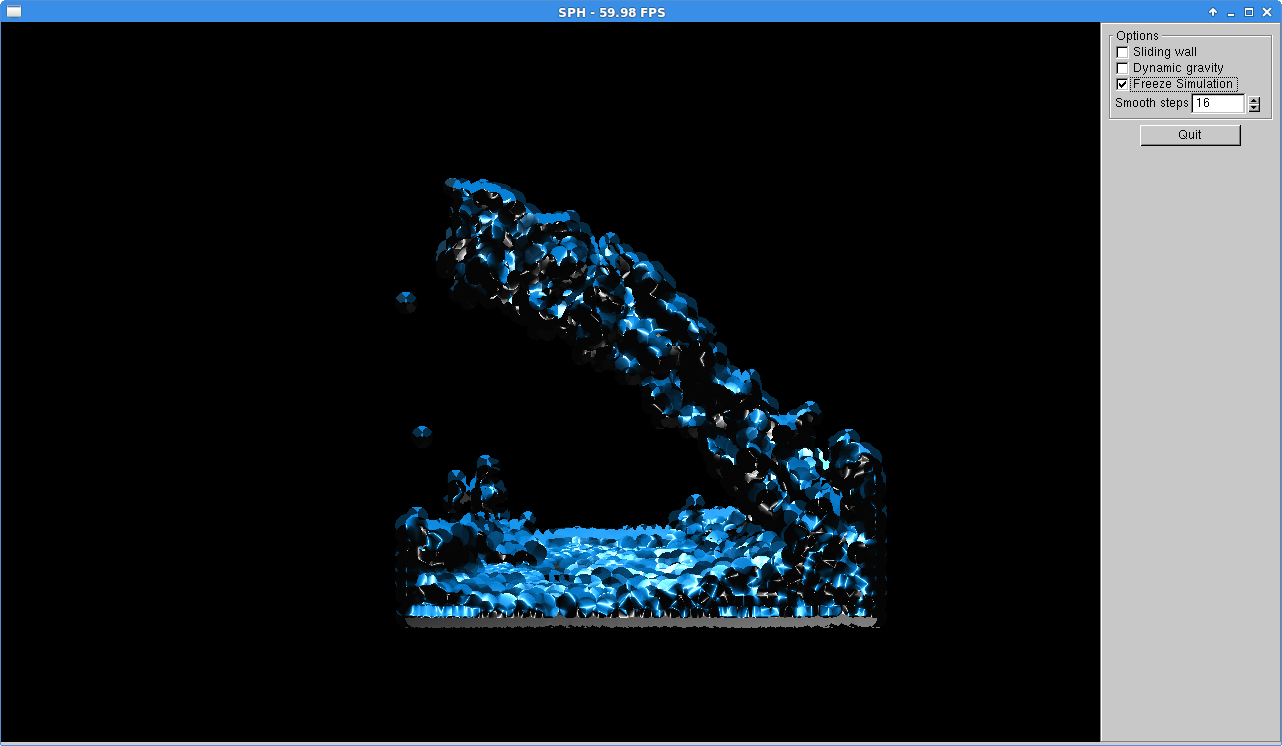
\includegraphics[width=0.48\textwidth,clip=true,trim=10cm 3cm 10cm 3cm]{pictures/colors.png}
\end{center}
\caption{The SPH simulation with splatted point and Phong and Fresnel rendering}
\label{fig:res} 
\vspace*{2ex}
\hrule
\end{figure}

Currently, splatting the points and determining the normals per fragment works. Also parts of the rendering implementation are complete, but refraction of the water is lacking.
Moreover, thickness is currently not implemented, as well as noise and foam.
Most notably lacking is the smoothing pass. 